\chapter{DPG and hyperbolic systems}

It is well-known that solutions to the pure convection equation
\[
\div \LRp{\beta u} = f
\]
are continuous in the distributional sense \emph{only along the streamline $\beta$}. As a consequence, several common physical phenomena that are commonly modeled using the convection equation are ill-posed, mathematically speaking. 

\section{Convection}
\seclab{sec:convDPG}

A common test problem with convection codes is $\beta = (-y,x)^T$, or the vortex problem described by Figure~\ref{fig:convCirc}. A rotating streamline convects material in a circular manner from the inflow boundaries around a square domain. However, along any \emph{closed loop} streamline, the solution is undefined, as there is no 

\begin{figure}[!h]
\centering
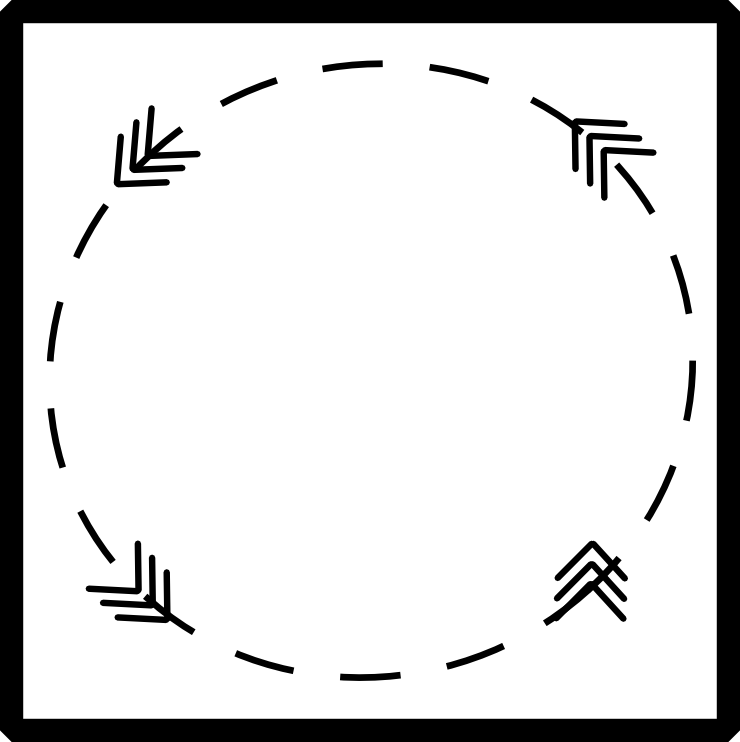
\includegraphics[scale = .25]{figs/convCirc.png}
\caption{Setup for the vortex problem.}
\label{fig:convCirc}
\end{figure}


\begin{figure}[!h]
\centering
\subfigure[Solution]{
\includegraphics[scale = .35]{figs/vortex.png}}
\subfigure[Mesh]{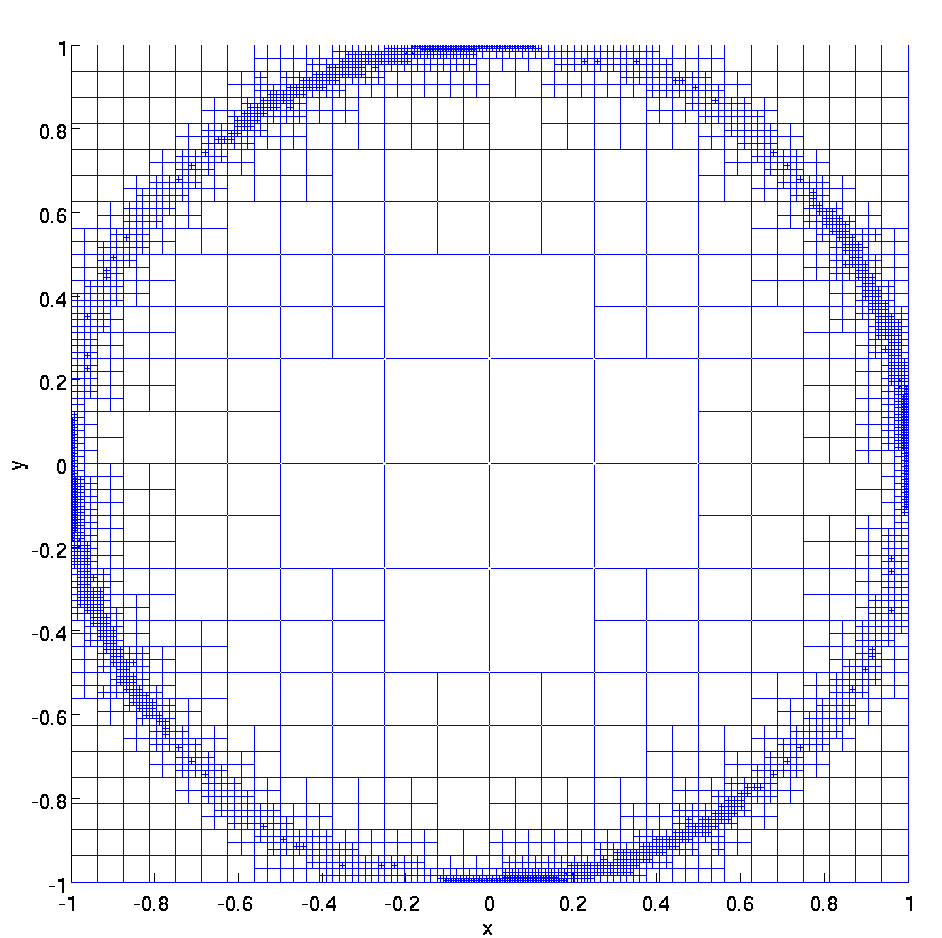
\includegraphics[scale = .35]{figs/vortexMesh.png}}
\caption{Regularized solution and mesh for the vortex problem.}
\label{fig:convCircResults}
\end{figure}

\subsection{Ill-posedness of fluxes}

Another issue with the discrete ultra-weak formulation is the ill-posedness of the fluxes on the mesh skeleton. Recall that the DPG formulation for convection is
\[
b(u,v) = \LRa{\widehat{f}_n, v} - \LRp{u,\beta\cdot \grad v} = \LRp{f,v}
\]
where $\widehat{f}_n$ represents the quantity $\beta_n u$. Since there is no small parameter $\epsilon$, as with convection-diffusion, we can use the quasi-optimal test norm 
\[
\nor{v}_V = \nor{\beta\cdot \grad v} + \nor{v}
\]
without worrying about approximability of test functions under this test norm. 

However, in directions orthogonal to the streamline, $\beta_n = 0$. Under the quasi-optimal test norm, there is no trace defined in the crossstream direction --- in other words, the flux $\widehat{f}_n$ is undefined on element edges such that $\beta_n = 0$. 

In numerical experiments, we took $\beta = (1,0)$, with a uniform mesh on $\Omega = [0,1]^2$. We took an inflow condition $u_0$ such that the best approximation error in the trial space was zero. The result of the ill-posedness of the ultra-weak formulation was that the error in the fluxes was $O(1e-8)$, whereas the error in the fluxes for exactly representable solutions to well-posed problems has typically been $O(1e-12)$ to $O(1e-14)$. 

\section{Linearized Euler}
\seclab{sec:eulerDPG}
The effect of the ill-posedness of fluxes can be seen more clearly for systems of hyperbolic equations. We take the linearized Euler equations as an example to illustrate such effects. 

The homogeneous Euler equations can be written in the form
\[
F_i(U)_{,i} = 0.
\]
Linearizing around constant $U_i$, $k = \ldots 4$, we arrive at the linearized Euler equations 
\[
\left(A_i(U)\Delta U\right)_{,i} = 0
\]
where $A_i(U)$ are the Euler Jacobian matrices. The exact solution to the above linearized Euler equations is illustrated in Figure~\ref{fig:linEulerExact}. \todo{explain why its exact sol}

\begin{figure}[!h]
\centering
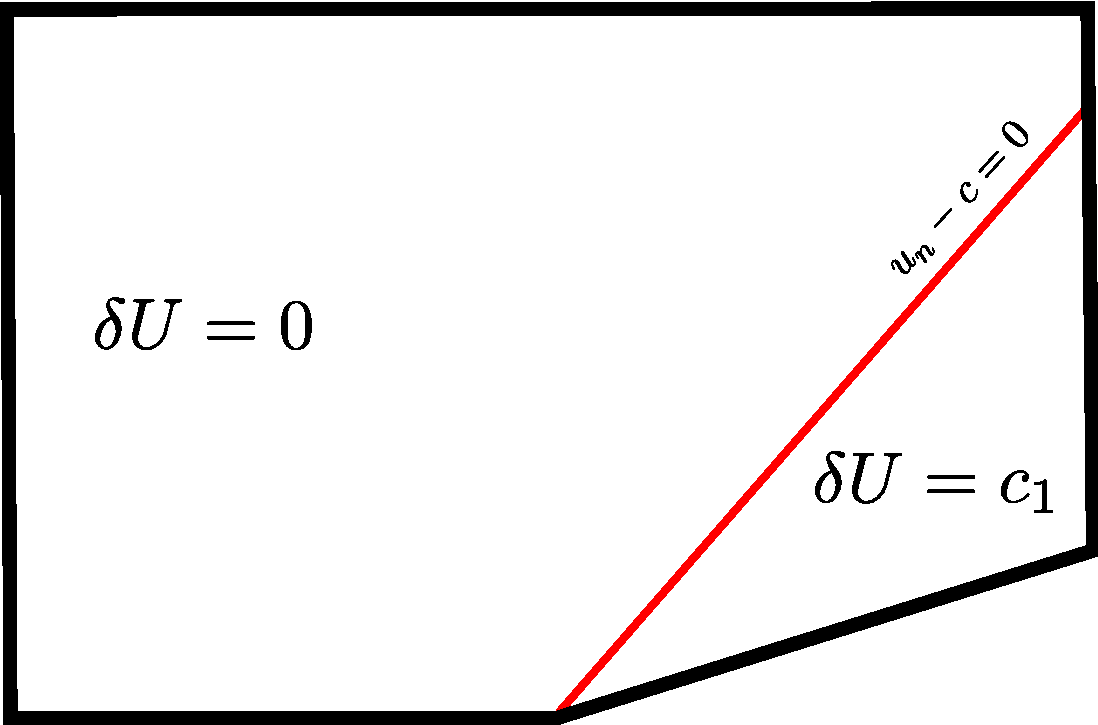
\includegraphics[scale = .5]{figs/linEulerExact.pdf}
\caption{Exact solution to linearized Euler for constant background flow.}
\label{fig:linEulerExact}
\end{figure}

In index notation, the linearized Euler equations can be written as
\[
\left(A_{i}(U)_{jk}\Delta U_k\right)_{,i} = 0
\]
Then, for test functions $V_j$, $j = 1,\ldots, 4$, the DPG formulation for the linearized Euler equations is 
\[
b(U,V) = \LRa{\widehat{f}_{j,n}, V_j} - \LRp{U_k,A_{i}(U)_{jk} V_{j,i}} = \LRp{f,v}
\]
where $f_{j,n}$ represents the quantity $A_n u_k$, where $A_n(U) = A_i(U)_{jk}n_i$ is the normal Euler Jacobian.

It is well-known that the normal Euler Jacobian\todo{finish}


\begin{figure}[!h]
\centering
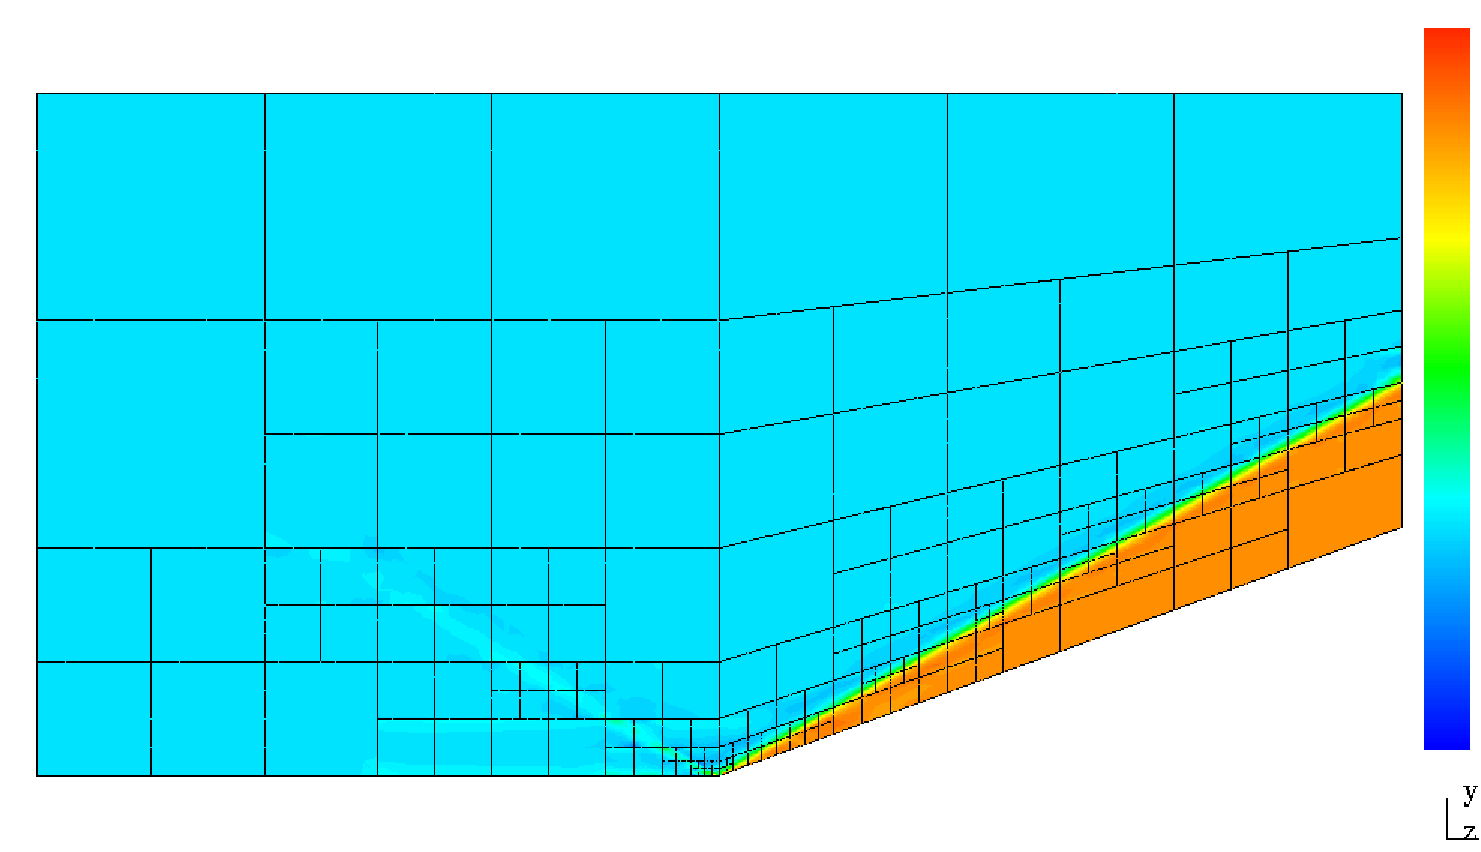
\includegraphics[scale = .5]{figs/sonicLines.pdf}
\caption{Sonic lines in the solution of the linearized Euler equations.}
\label{fig:linEulerResults}
\end{figure}
